\section{补充图}

为把正文与参考文献控制在提交页数以内，下列示意图与对照图改置于本附录。
各图仍由正文引用，编号连续，结论与数据口径不变。

\begin{figure}[H]
  \centering
  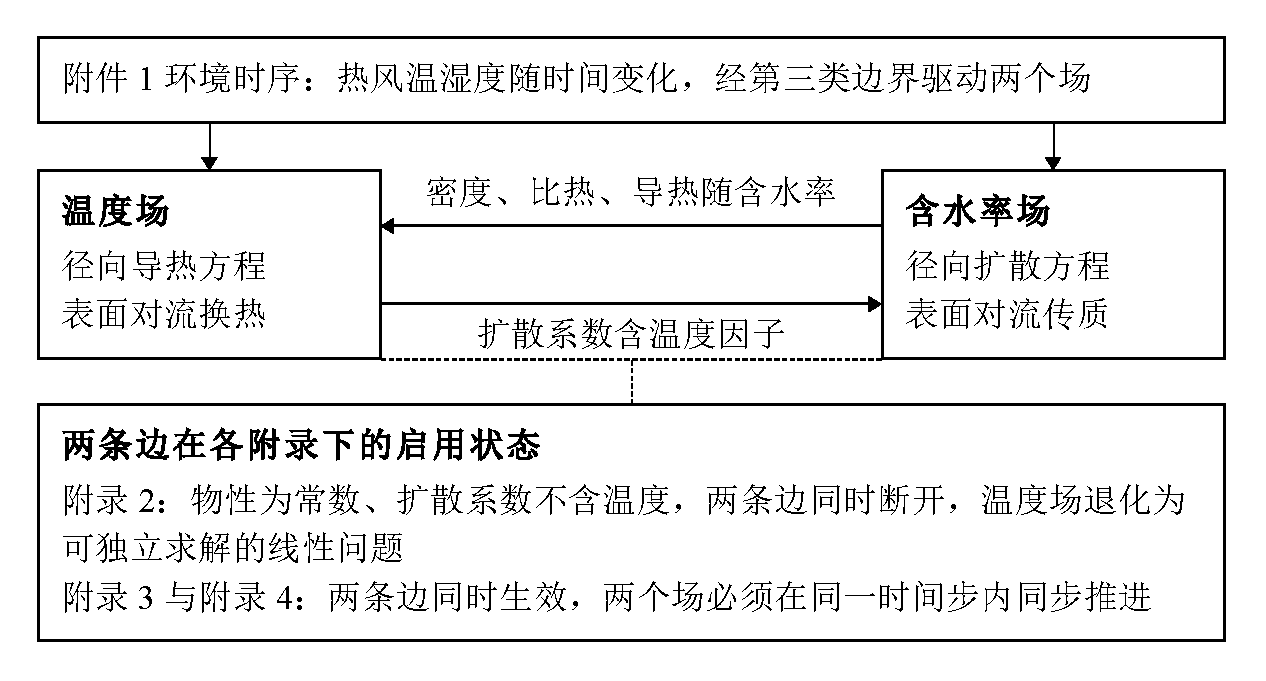
\includegraphics[width=0.70\textwidth,height=0.40\textheight,keepaspectratio]{../figures/fig_coupling_structure.pdf}
  \caption{温度场与含水率场的耦合结构}
  \label{fig:coupling_structure}
\end{figure}

\begin{figure}[H]
  \centering
  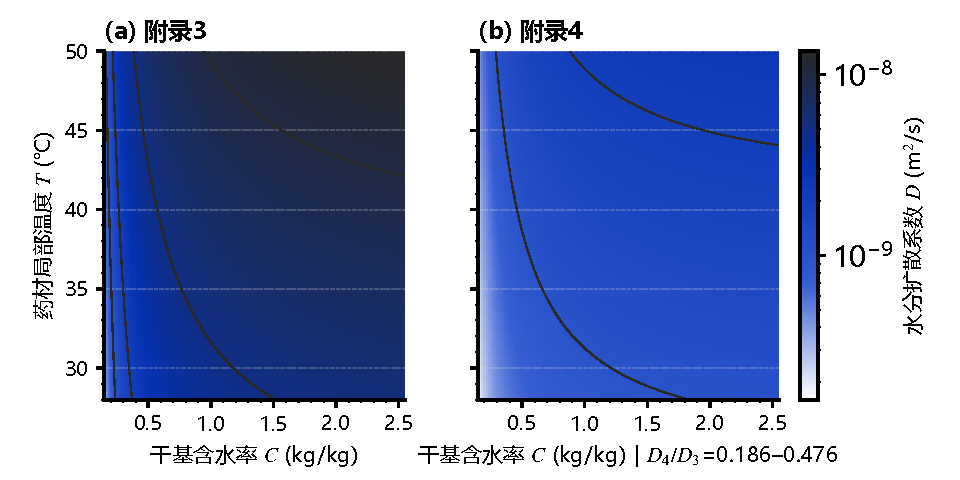
\includegraphics[width=0.78\textwidth,height=0.38\textheight,keepaspectratio]{../figures/fig_property_maps.pdf}
  \caption{附录 3 与附录 4 的水分扩散系数分布对比}
  \label{fig:property_maps}
\end{figure}

\begin{figure}[H]
  \centering
  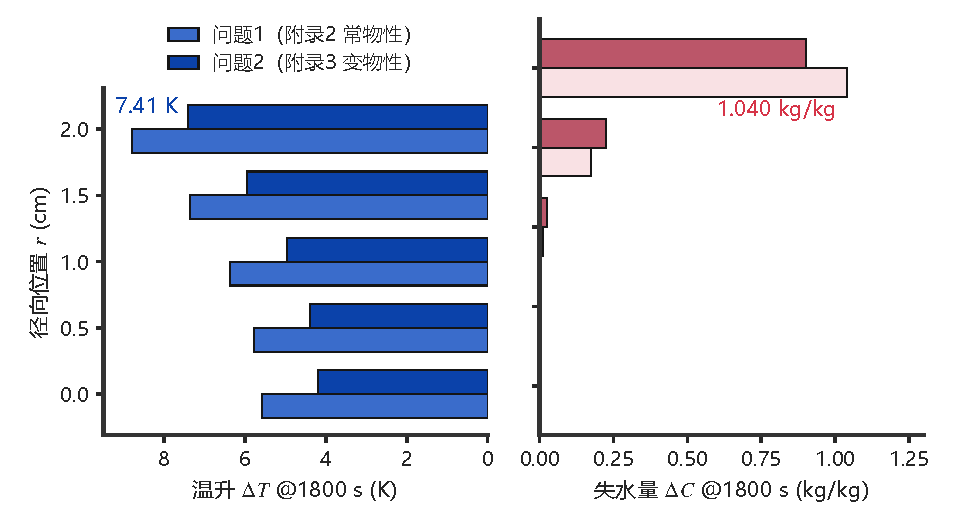
\includegraphics[width=0.86\textwidth,height=0.32\textheight,keepaspectratio]{../figures/fig_q12_contrast.pdf}
  \caption{问题一与问题二在 $t=1800$~s 的增量对比}
  \label{fig:q12_contrast}
\end{figure}

\begin{figure}[H]
  \centering
  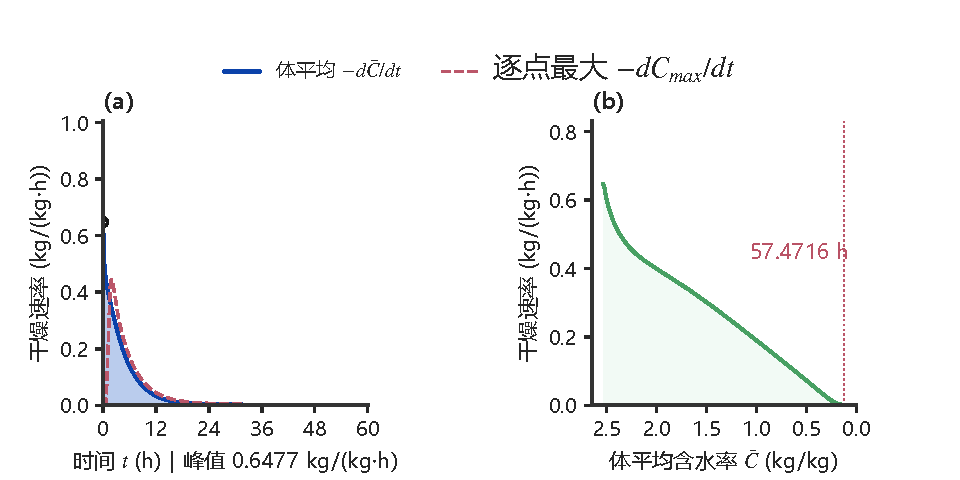
\includegraphics[width=0.88\textwidth,height=0.32\textheight,keepaspectratio]{../figures/fig_q3_rate_curve.pdf}
  \caption{问题三干燥速率的两种读法}
  \label{fig:q3_rate_curve}
\end{figure}

\begin{figure}[H]
  \centering
  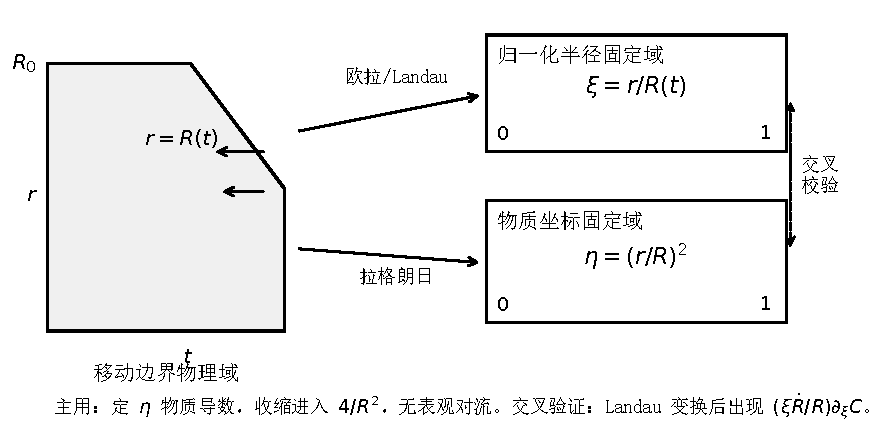
\includegraphics[width=0.55\textwidth,height=0.36\textheight,keepaspectratio]{../figures/tikz_landau_map.pdf}
  \caption{归一化坐标把收缩物理域映为固定计算域}
  \label{fig:landau_map}
\end{figure}

\begin{figure}[H]
  \centering
  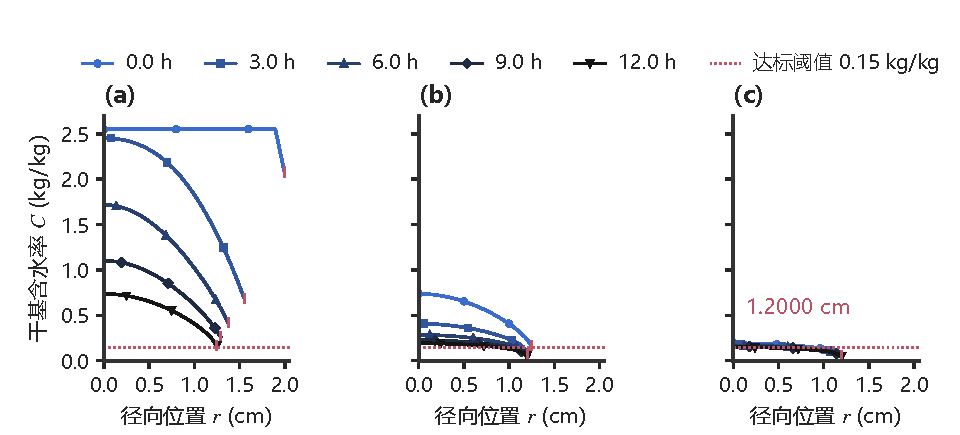
\includegraphics[width=0.88\textwidth,height=0.32\textheight,keepaspectratio]{../figures/fig_q4_triptych.pdf}
  \caption{问题四含水率剖面的三阶段演化}
  \label{fig:q4_triptych}
\end{figure}

\begin{figure}[H]
  \centering
  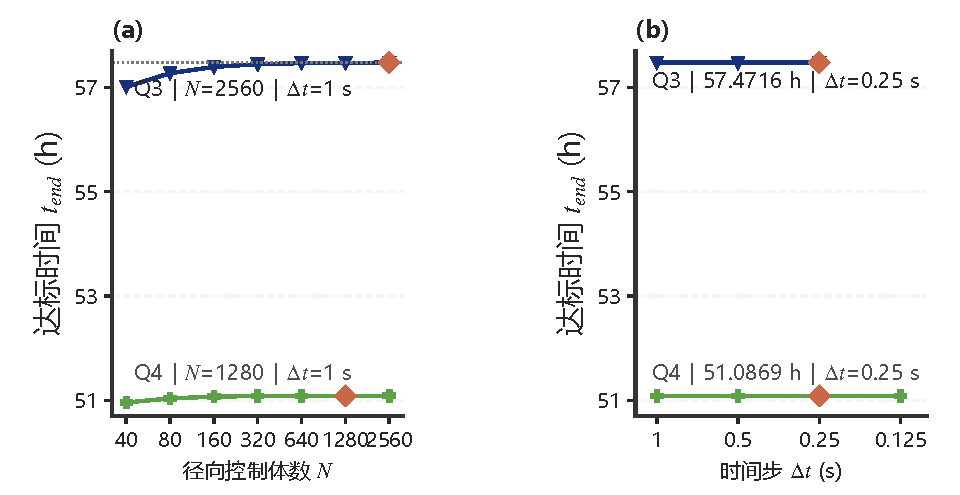
\includegraphics[width=0.78\textwidth,height=0.34\textheight,keepaspectratio]{../figures/fig_convergence.pdf}
  \caption{问题三与问题四的空间和时间步收敛性}
  \label{fig:convergence}
\end{figure}
